\section{Task 3 --- Performance Across Database Sizes}

\subsection{Measurement protocol}
We run each of Q1--Q6 five times at each of the five cumulative sizes, giving 150 timing records in \path{Task 3/results/task3_measurements.csv}. The measurement loop has no separate warm-up, although the notebook executes the queries in its earlier results section.
Runtime is the client-observed time around SQL execution and fetching all result rows.
Database size and housing size are recorded with each block in the measurement file; Table~\ref{tab:t3perf} uses the per-step averages from \texttt{task3\_summary.csv}.
The later Task~4 environment snapshot records PostgreSQL~18.4 on macOS arm64 with 10 CPUs. Task~3 has no equivalent saved environment snapshot, so we cannot verify every setting against that later record.

\subsection{Average runtime by size}
Table~\ref{tab:t3perf} reports mean runtime in milliseconds (five runs).
Figure~\ref{fig:t3chart} plots runtime against database size for each query.

\begin{table}[H]
\centering
\caption{Mean runtime (ms) of Q1--Q6 over five timed runs at each database size. Sales and DB size from \texttt{task3\_summary.csv}.}
\label{tab:t3perf}
\footnotesize
\begin{tabular}{@{}rrrrrrrrr@{}}
\toprule
Step & Sales & DB (MB) & Q1 & Q2 & Q3 & Q4 & Q5 & Q6 \\
\midrule
1 & 241{,}483 & 44.18 & 22.40 & 163.38 & 40.53 & 39.77 & 93.44 & 34.61 \\
2 & 278{,}636 & 47.54 & 23.29 & 193.04 & 47.80 & 44.16 & 106.37 & 34.97 \\
3 & 330{,}839 & 53.73 & 20.96 & 231.12 & 68.88 & 47.55 & 126.10 & 30.98 \\
4 & 700{,}490 & 83.03 & 20.81 & 314.67 & 141.08 & 58.42 & 155.28 & 31.38 \\
5 & 987{,}686 & 104.87 & 22.28 & 412.19 & 217.83 & 70.58 & 226.61 & 33.47 \\
\bottomrule
\end{tabular}
\end{table}

\begin{figure}[H]
\centering
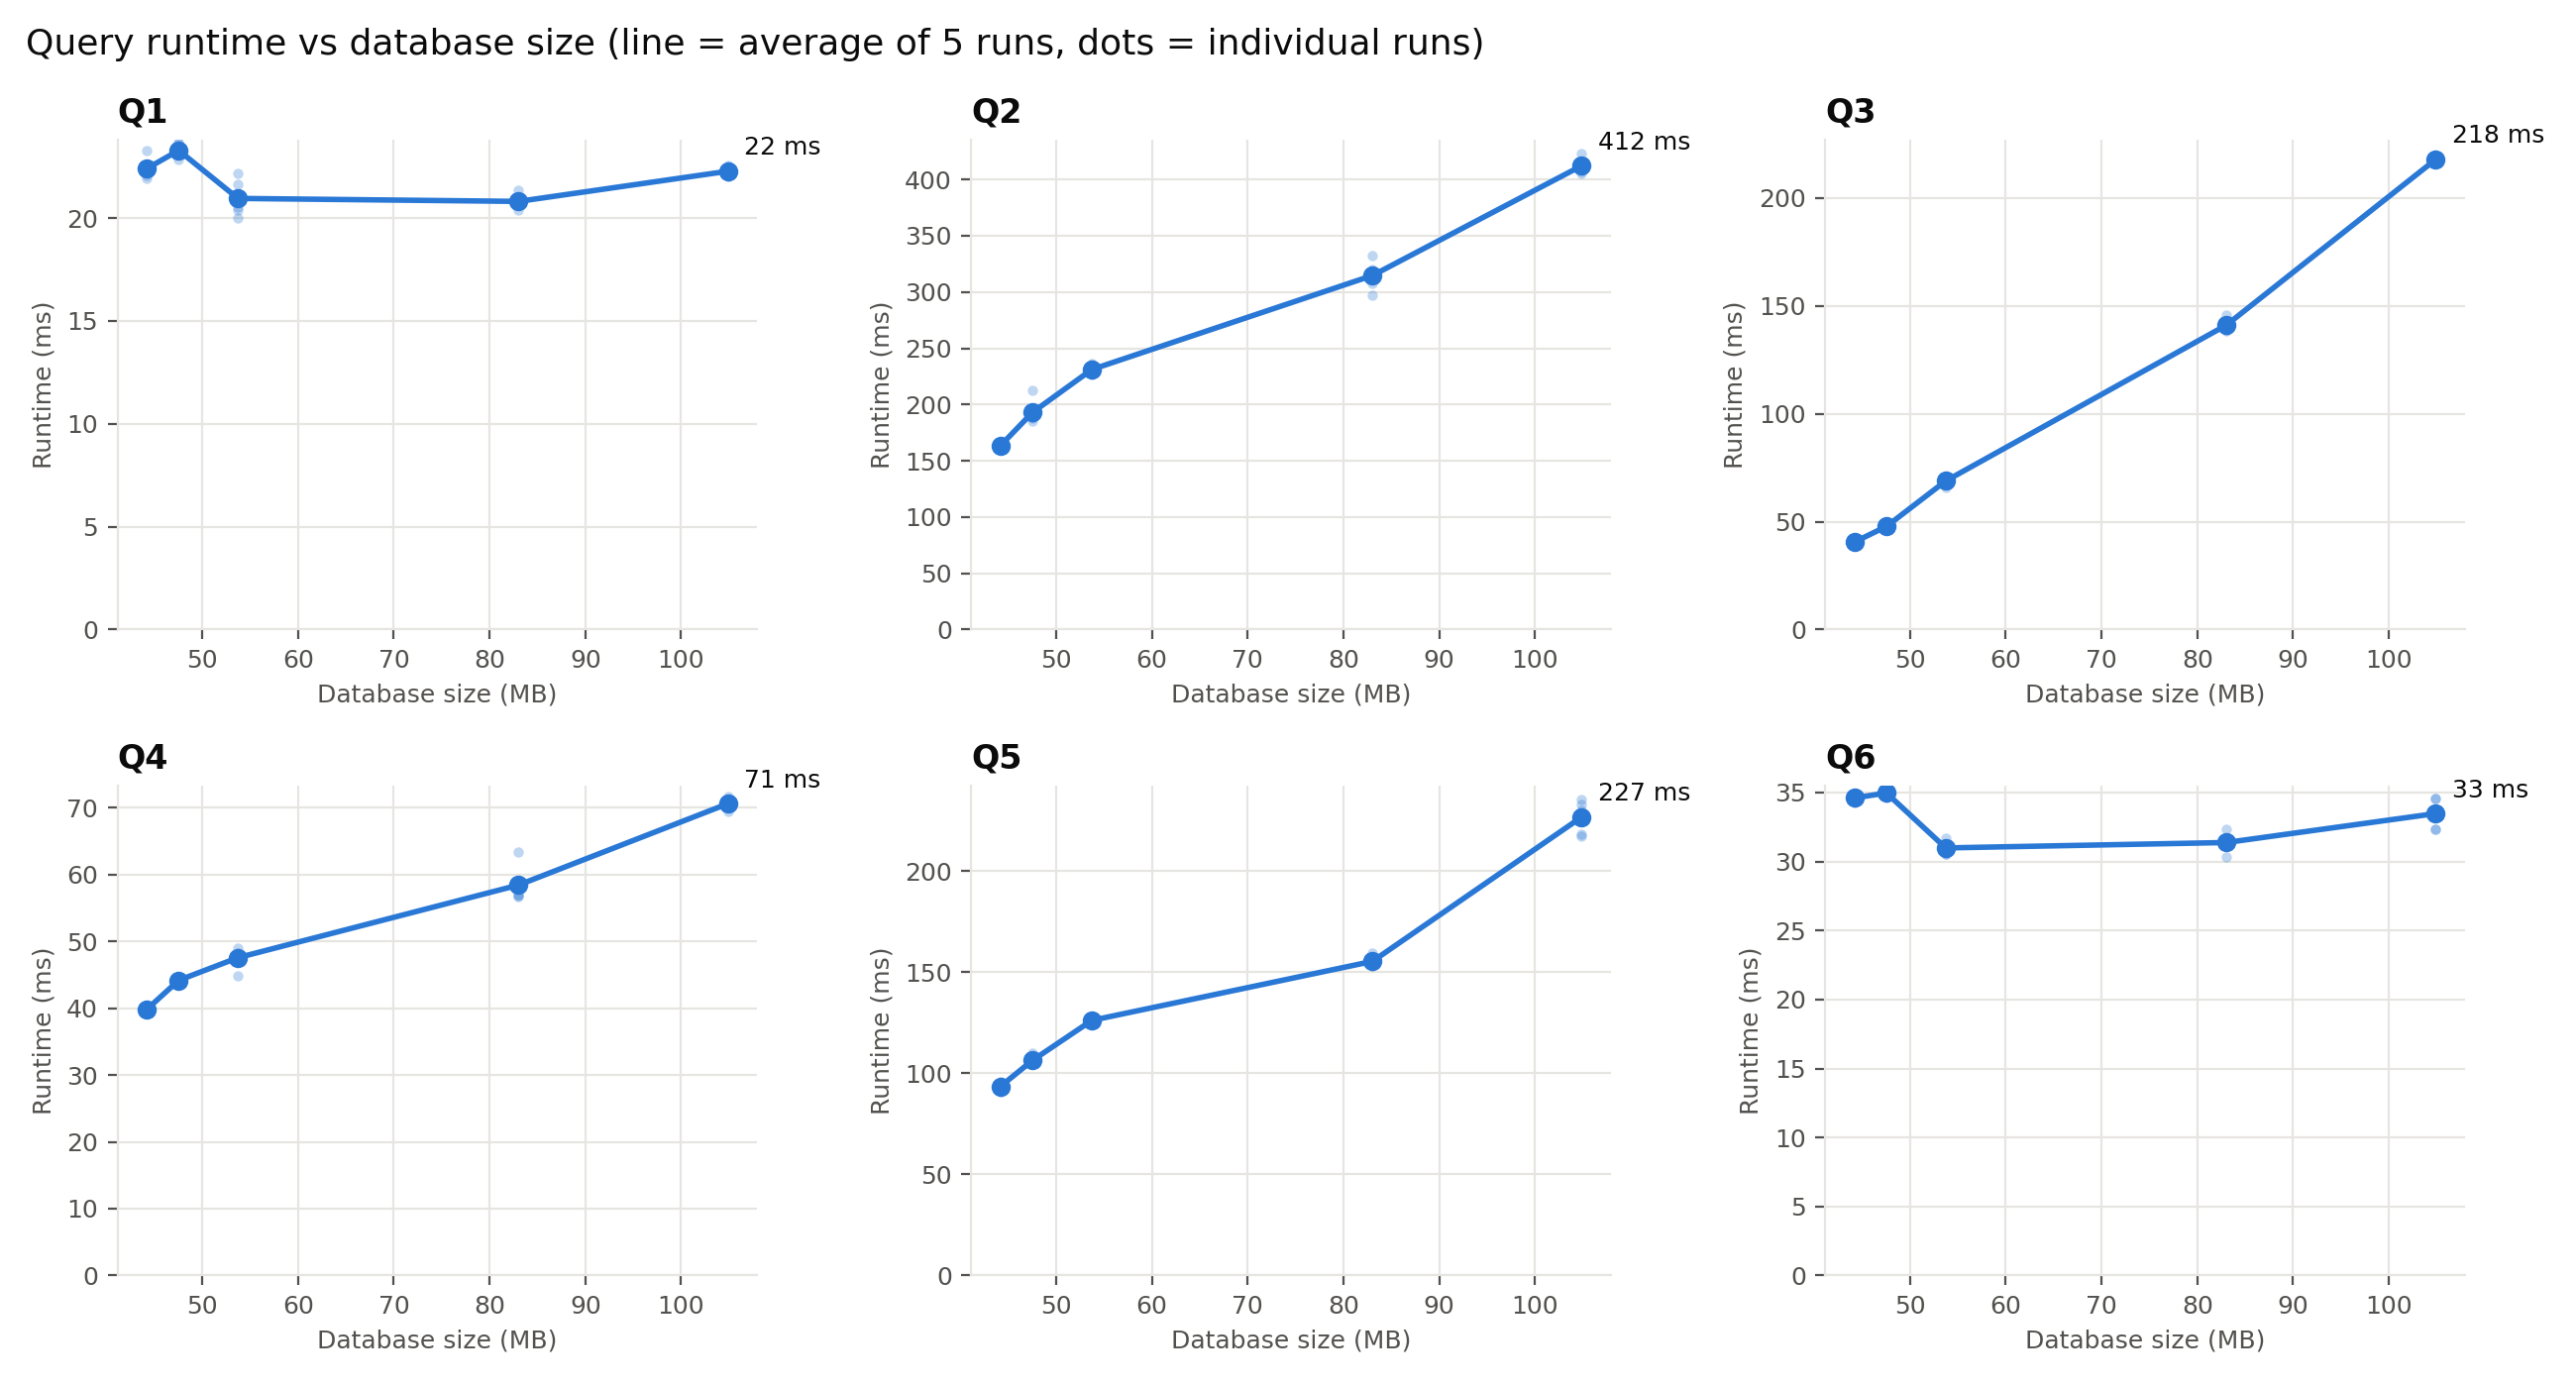
\includegraphics[width=\textwidth]{figures/task3_runtime_vs_size.png}
\caption{Query runtime versus database size (Task~3). Lines connect the five-run means, and dots show individual runs.}
\label{fig:t3chart}
\end{figure}

\subsection{Discussion}
\paragraph{Observed scaling.}
From step~1 to step~5, sales grow by about $4.1\times$ while database size roughly doubles.
Q2 and Q3 grow strongly with size (Q2 about $2.5\times$, Q3 about $5.4\times$).
Q4 and Q5 grow more slowly than the sales count.
Q1 remains around 21--23~ms and Q6 around 31--35~ms.

\paragraph{Execution plans.}
Saved Task~4 \texttt{EXPLAIN} plans on the largest database (without the Task~4 index) show that Q1 and Q6 apply a date filter on \texttt{resale\_transaction} and use parallel sequential scans, keeping only about 8.1\% of sales for 2022--2024.
Q2--Q5 read essentially all sales; Q3's \texttt{WITH three\_room} is referenced twice and is materialised, and Q2's large sort spills to disk under default \texttt{work\_mem} (see Task~4 supporting experiments).
The added files contain older sales outside the Q1/Q6 date window, so their selected transaction sets remain fixed. Parallel scans may also help keep their runtimes low. The saved plans explain the work performed on the largest database, while cache effects and background load across the five measurements remain unmeasured.

\paragraph{Implication for indexing.}
Task~3 suggested Q2 and Q3 as first index candidates because they dominate absolute runtime.
Task~4 tests whether indexes can reduce this work. The clearest improvement comes from indexing the date filter in Q1.
